\documentclass[tikz,border=6pt]{standalone}
\usepackage[T1]{fontenc}
\usepackage{lmodern}
\usepackage{tikz}
\usetikzlibrary{arrows.meta,calc}

\definecolor{itink}{RGB}{38,45,53}
\definecolor{itblue}{RGB}{39,126,185}
\definecolor{itgreen}{RGB}{45,139,111}
\definecolor{itorange}{RGB}{204,101,42}
\definecolor{itred}{RGB}{200,64,50}
\definecolor{itgray}{RGB}{245,247,249}

\begin{document}
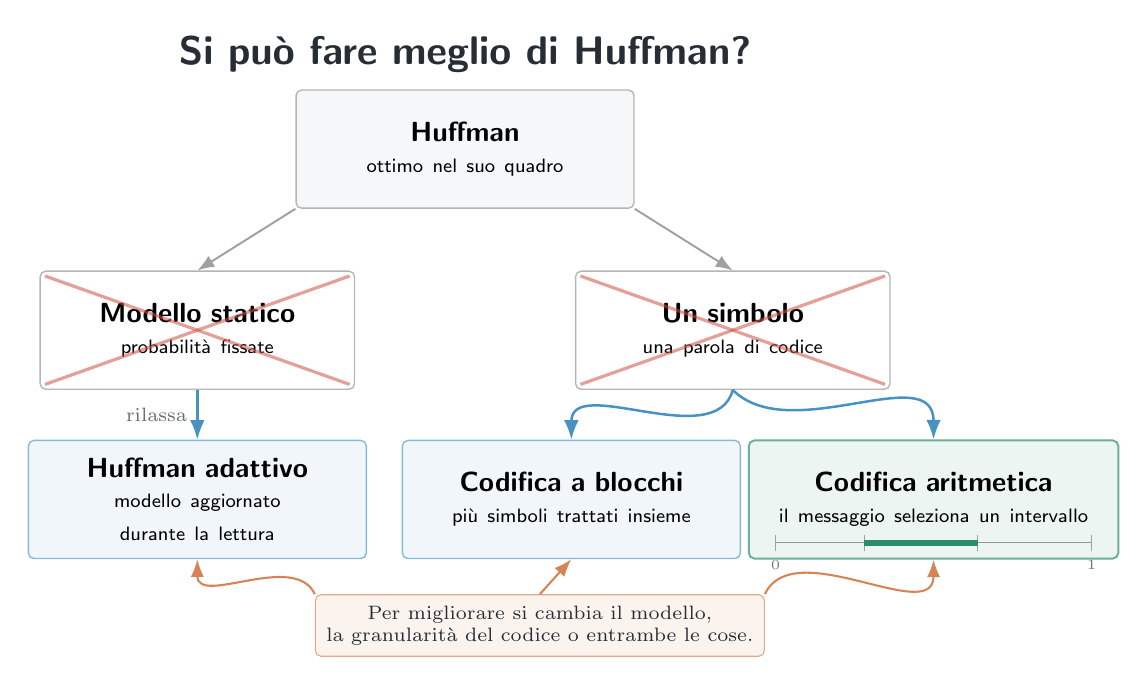
\begin{tikzpicture}[
    font=\sffamily,
    >=Latex,
    % Box styles: the figure contrasts Huffman's framework with the ways out.
    box/.style={
        draw=itink!35,
        line width=0.5pt,
        rounded corners=2pt,
        align=center,
        inner xsep=7pt,
        inner ysep=6pt,
        minimum height=15mm,
        fill=white
    },
    source/.style={
        box,
        fill=itgray,
        text width=38mm
    },
    constraint/.style={
        box,
        text width=35mm
    },
    method/.style={
        box,
        draw=itblue!55,
        fill=itblue!7,
        text width=38mm
    },
    highlight/.style={
        method,
        draw=itgreen!70,
        fill=itgreen!9,
        line width=0.7pt,
        text width=42mm
    },
    arrow/.style={->, line width=0.9pt, draw=itblue!85},
    weakarrow/.style={->, line width=0.7pt, draw=itink!45},
    cross/.style={line width=1.15pt, draw=itred!90, opacity=0.55}
]
    \node[font=\sffamily\bfseries\Large, text=itink] (question) at (0,4.0)
        {Si pu\`o fare meglio di Huffman?};

    \node[source] (huffman) at (0,2.8)
        {\textbf{Huffman}\\[-1pt]\scriptsize ottimo nel suo quadro};

    \node[constraint] (static) at (-3.4,0.5)
        {\textbf{Modello statico}\\[-1pt]\scriptsize probabilit\`a fissate};
    \node[constraint] (symbol) at (3.4,0.5)
        {\textbf{Un simbolo}\\[-1pt]\scriptsize una parola di codice};

    \node[method] (adaptive) at (-3.4,-1.65)
        {\textbf{Huffman adattivo}\\[-1pt]\scriptsize modello aggiornato durante la lettura};
    \node[method] (block) at (1.35,-1.65)
        {\textbf{Codifica a blocchi}\\[-1pt]\scriptsize pi\`u simboli trattati insieme};
    \node[highlight] (arith) at (5.95,-1.65)
        {\textbf{Codifica aritmetica}\\[-1pt]\scriptsize il messaggio seleziona un intervallo};

    \draw[weakarrow] (huffman.south west) -- (static.north);
    \draw[weakarrow] (huffman.south east) -- (symbol.north);

    % The red strokes mark the constraints that are relaxed after Huffman.
    \draw[cross] ($(static.north west)+(2pt,-2pt)$) -- ($(static.south east)+(-2pt,2pt)$);
    \draw[cross] ($(static.south west)+(2pt,2pt)$) -- ($(static.north east)+(-2pt,-2pt)$);
    \draw[cross] ($(symbol.north west)+(2pt,-2pt)$) -- ($(symbol.south east)+(-2pt,2pt)$);
    \draw[cross] ($(symbol.south west)+(2pt,2pt)$) -- ($(symbol.north east)+(-2pt,-2pt)$);

    \draw[arrow] (static.south) --
        node[left, font=\scriptsize, text=itink!70] {rilassa} (adaptive.north);
    \draw[arrow] (symbol.south) to[out=-105,in=90] (block.north);
    \draw[arrow] (symbol.south) to[out=-45,in=90] (arith.north);

    % Small interval preview: arithmetic coding represents the whole message
    % by narrowing a subinterval of [0,1).
    \coordinate (intleft) at ($(arith.south west)+(10pt,6pt)$);
    \coordinate (intright) at ($(arith.south east)+(-10pt,6pt)$);
    \coordinate (inta) at ($(intleft)!0.28!(intright)$);
    \coordinate (intb) at ($(intleft)!0.64!(intright)$);
    \draw[itink!50, line width=0.4pt] (intleft) -- (intright);
    \foreach \p in {intleft,inta,intb,intright} {
        \draw[itink!45, line width=0.35pt] ($(\p)+(0,-3pt)$) -- ($(\p)+(0,3pt)$);
    }
    \draw[itgreen, line width=1.9pt] (inta) -- (intb);
    \node[font=\tiny, text=itink!65, anchor=north] at ($(intleft)+(0,-3pt)$) {$0$};
    \node[font=\tiny, text=itink!65, anchor=north] at ($(intright)+(0,-3pt)$) {$1$};

    \node[
        draw=itorange!55,
        fill=itorange!8,
        rounded corners=2pt,
        inner sep=4pt,
        align=center,
        font=\scriptsize,
        text=itink
    ] (note) at (0.95,-3.25)
        {Per migliorare si cambia il modello,\\la granularit\`a del codice o entrambe le cose.};

    \draw[->, draw=itorange!80, line width=0.75pt]
        (note.north west) to[out=115,in=-90] (adaptive.south);
    \draw[->, draw=itorange!80, line width=0.75pt]
        (note.north) -- (block.south);
    \draw[->, draw=itorange!80, line width=0.75pt]
        (note.north east) to[out=65,in=-90] (arith.south);
\end{tikzpicture}
\end{document}
